\section{Technical Approach}
\label{sec:TechnicalApproach}

\begin{figure}
\centering
\begin{subfigure}[b]{0.64\textwidth}
        \centering
        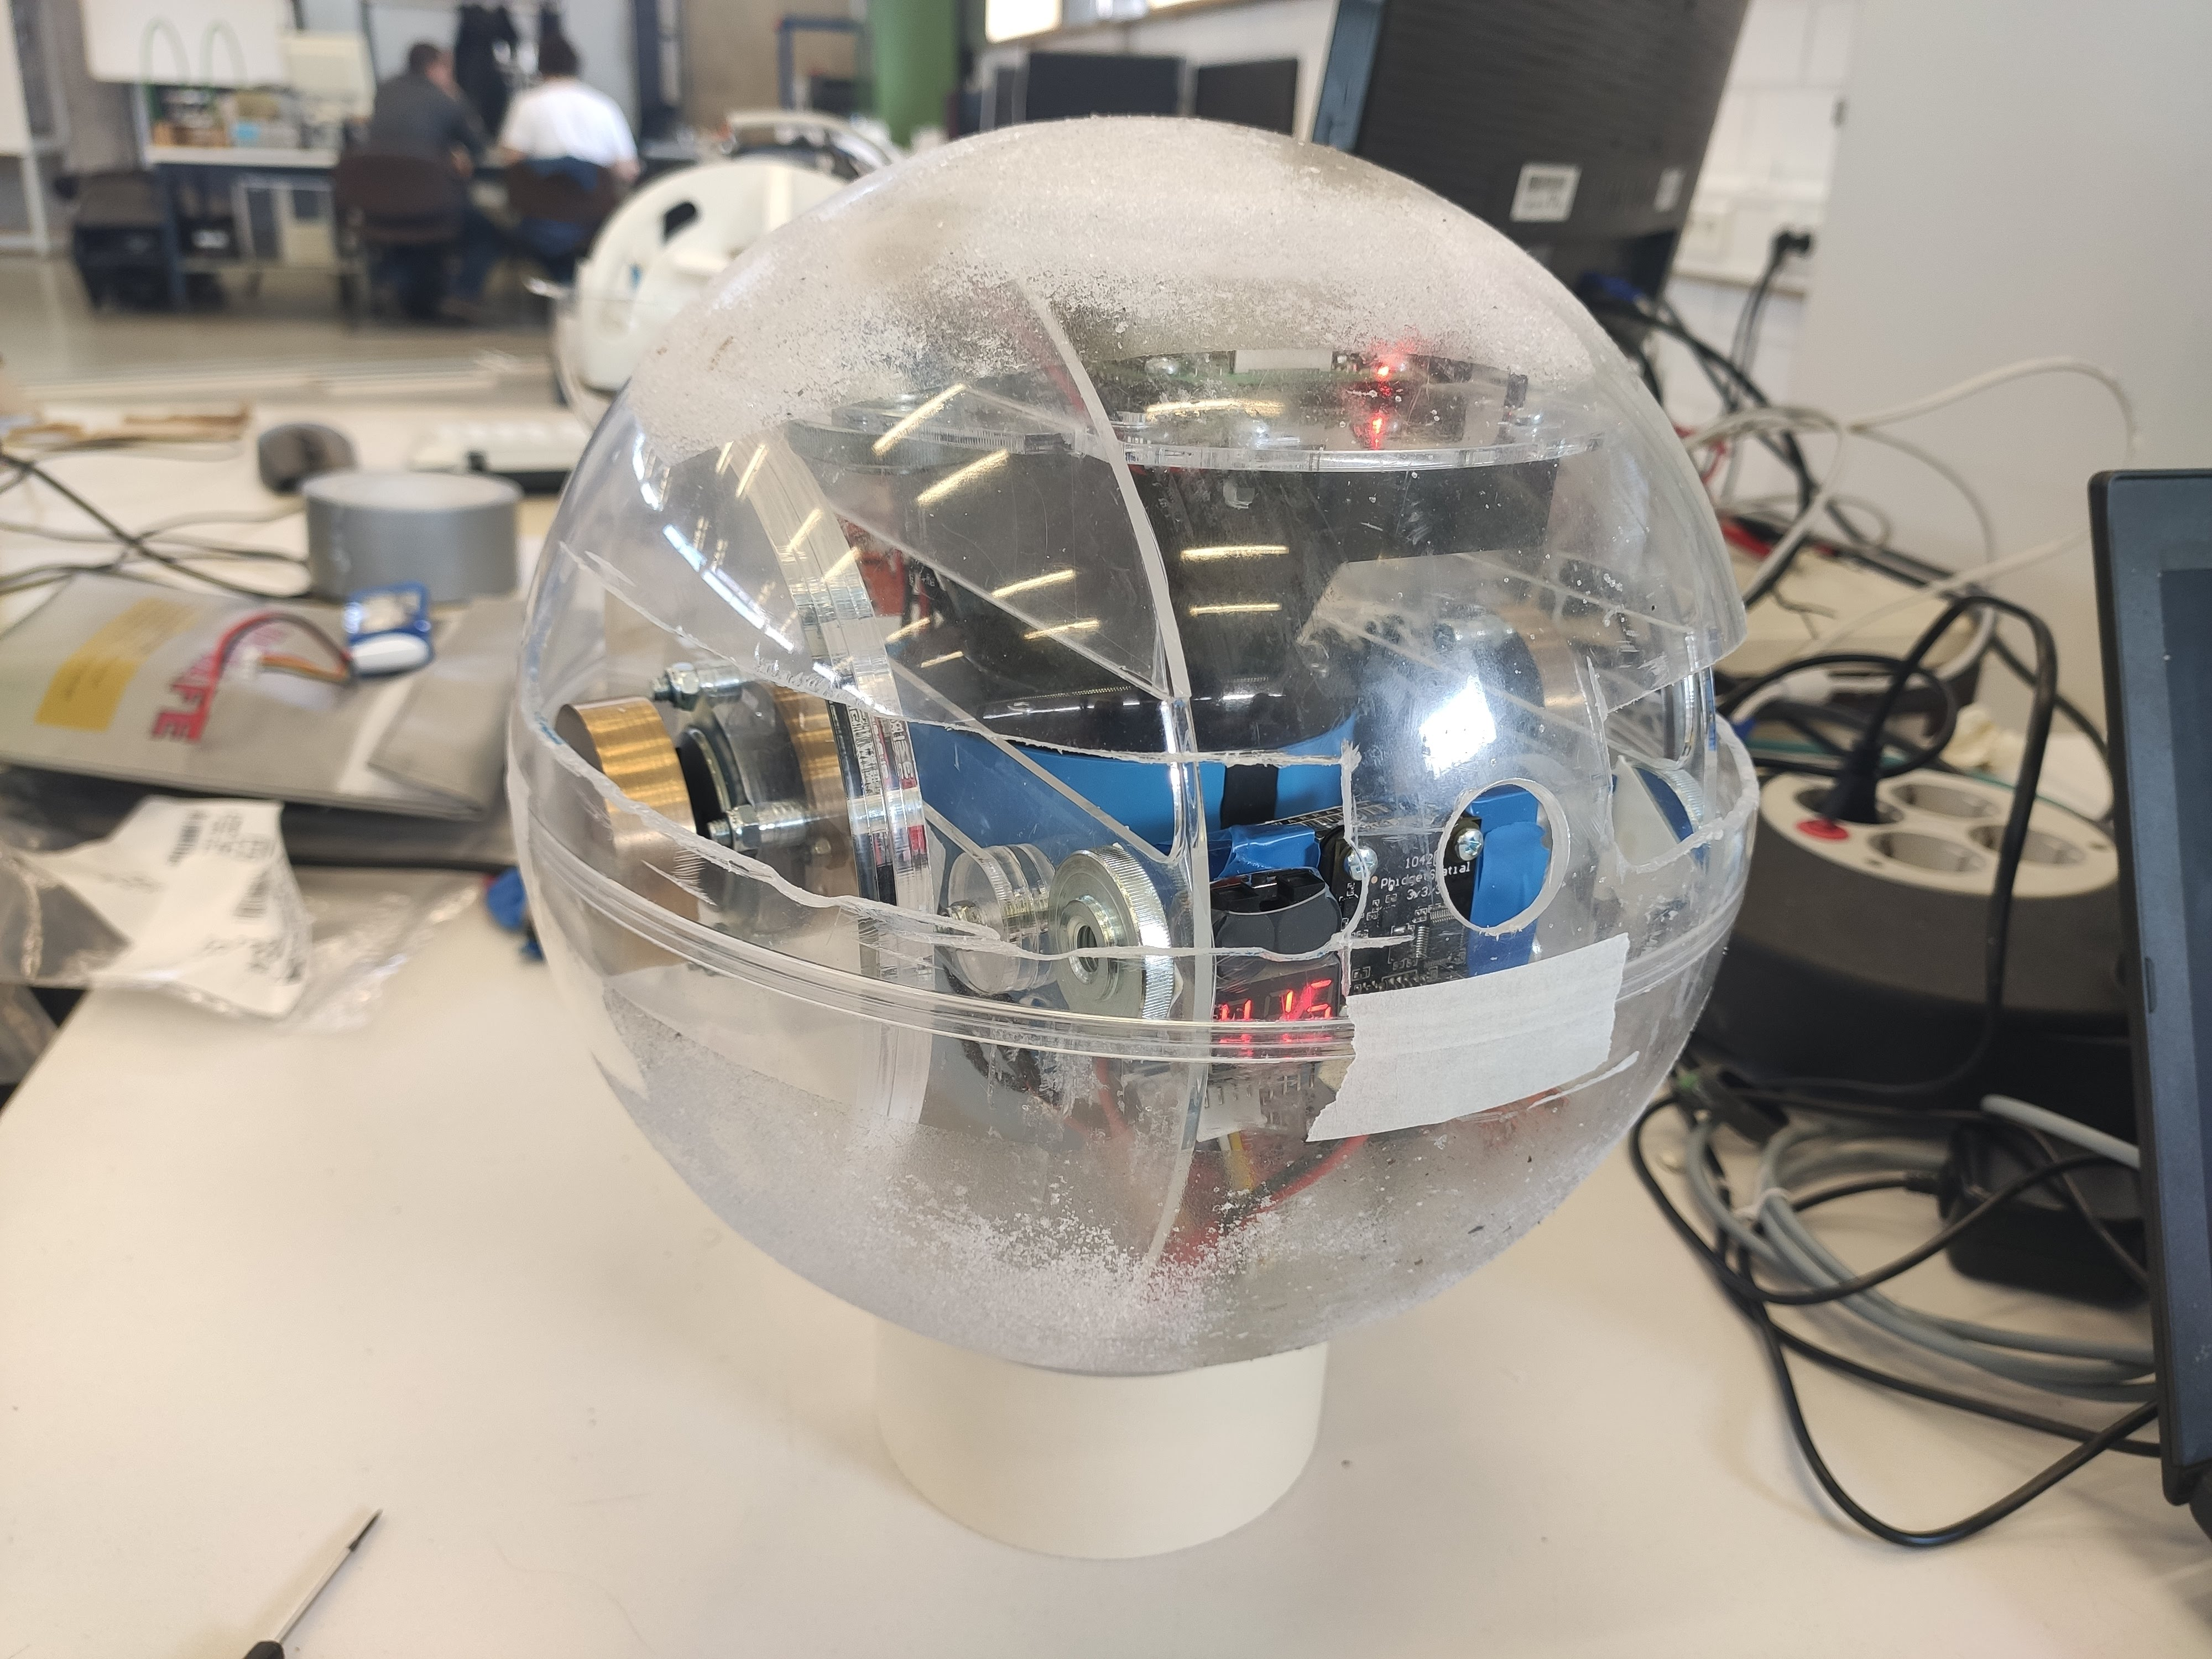
\includegraphics[width=\textwidth]{../Media/sphereFullshellLeft.jpg}
        \caption{Hardware setup of the L.U.N.A sphere prototype, including notches in the shell and friction granule.}
        \label{sec:TechnicalApproach:fig:prototype}
\end{subfigure}
\hfill
\begin{subfigure}[b]{0.34\textwidth}
        \centering
        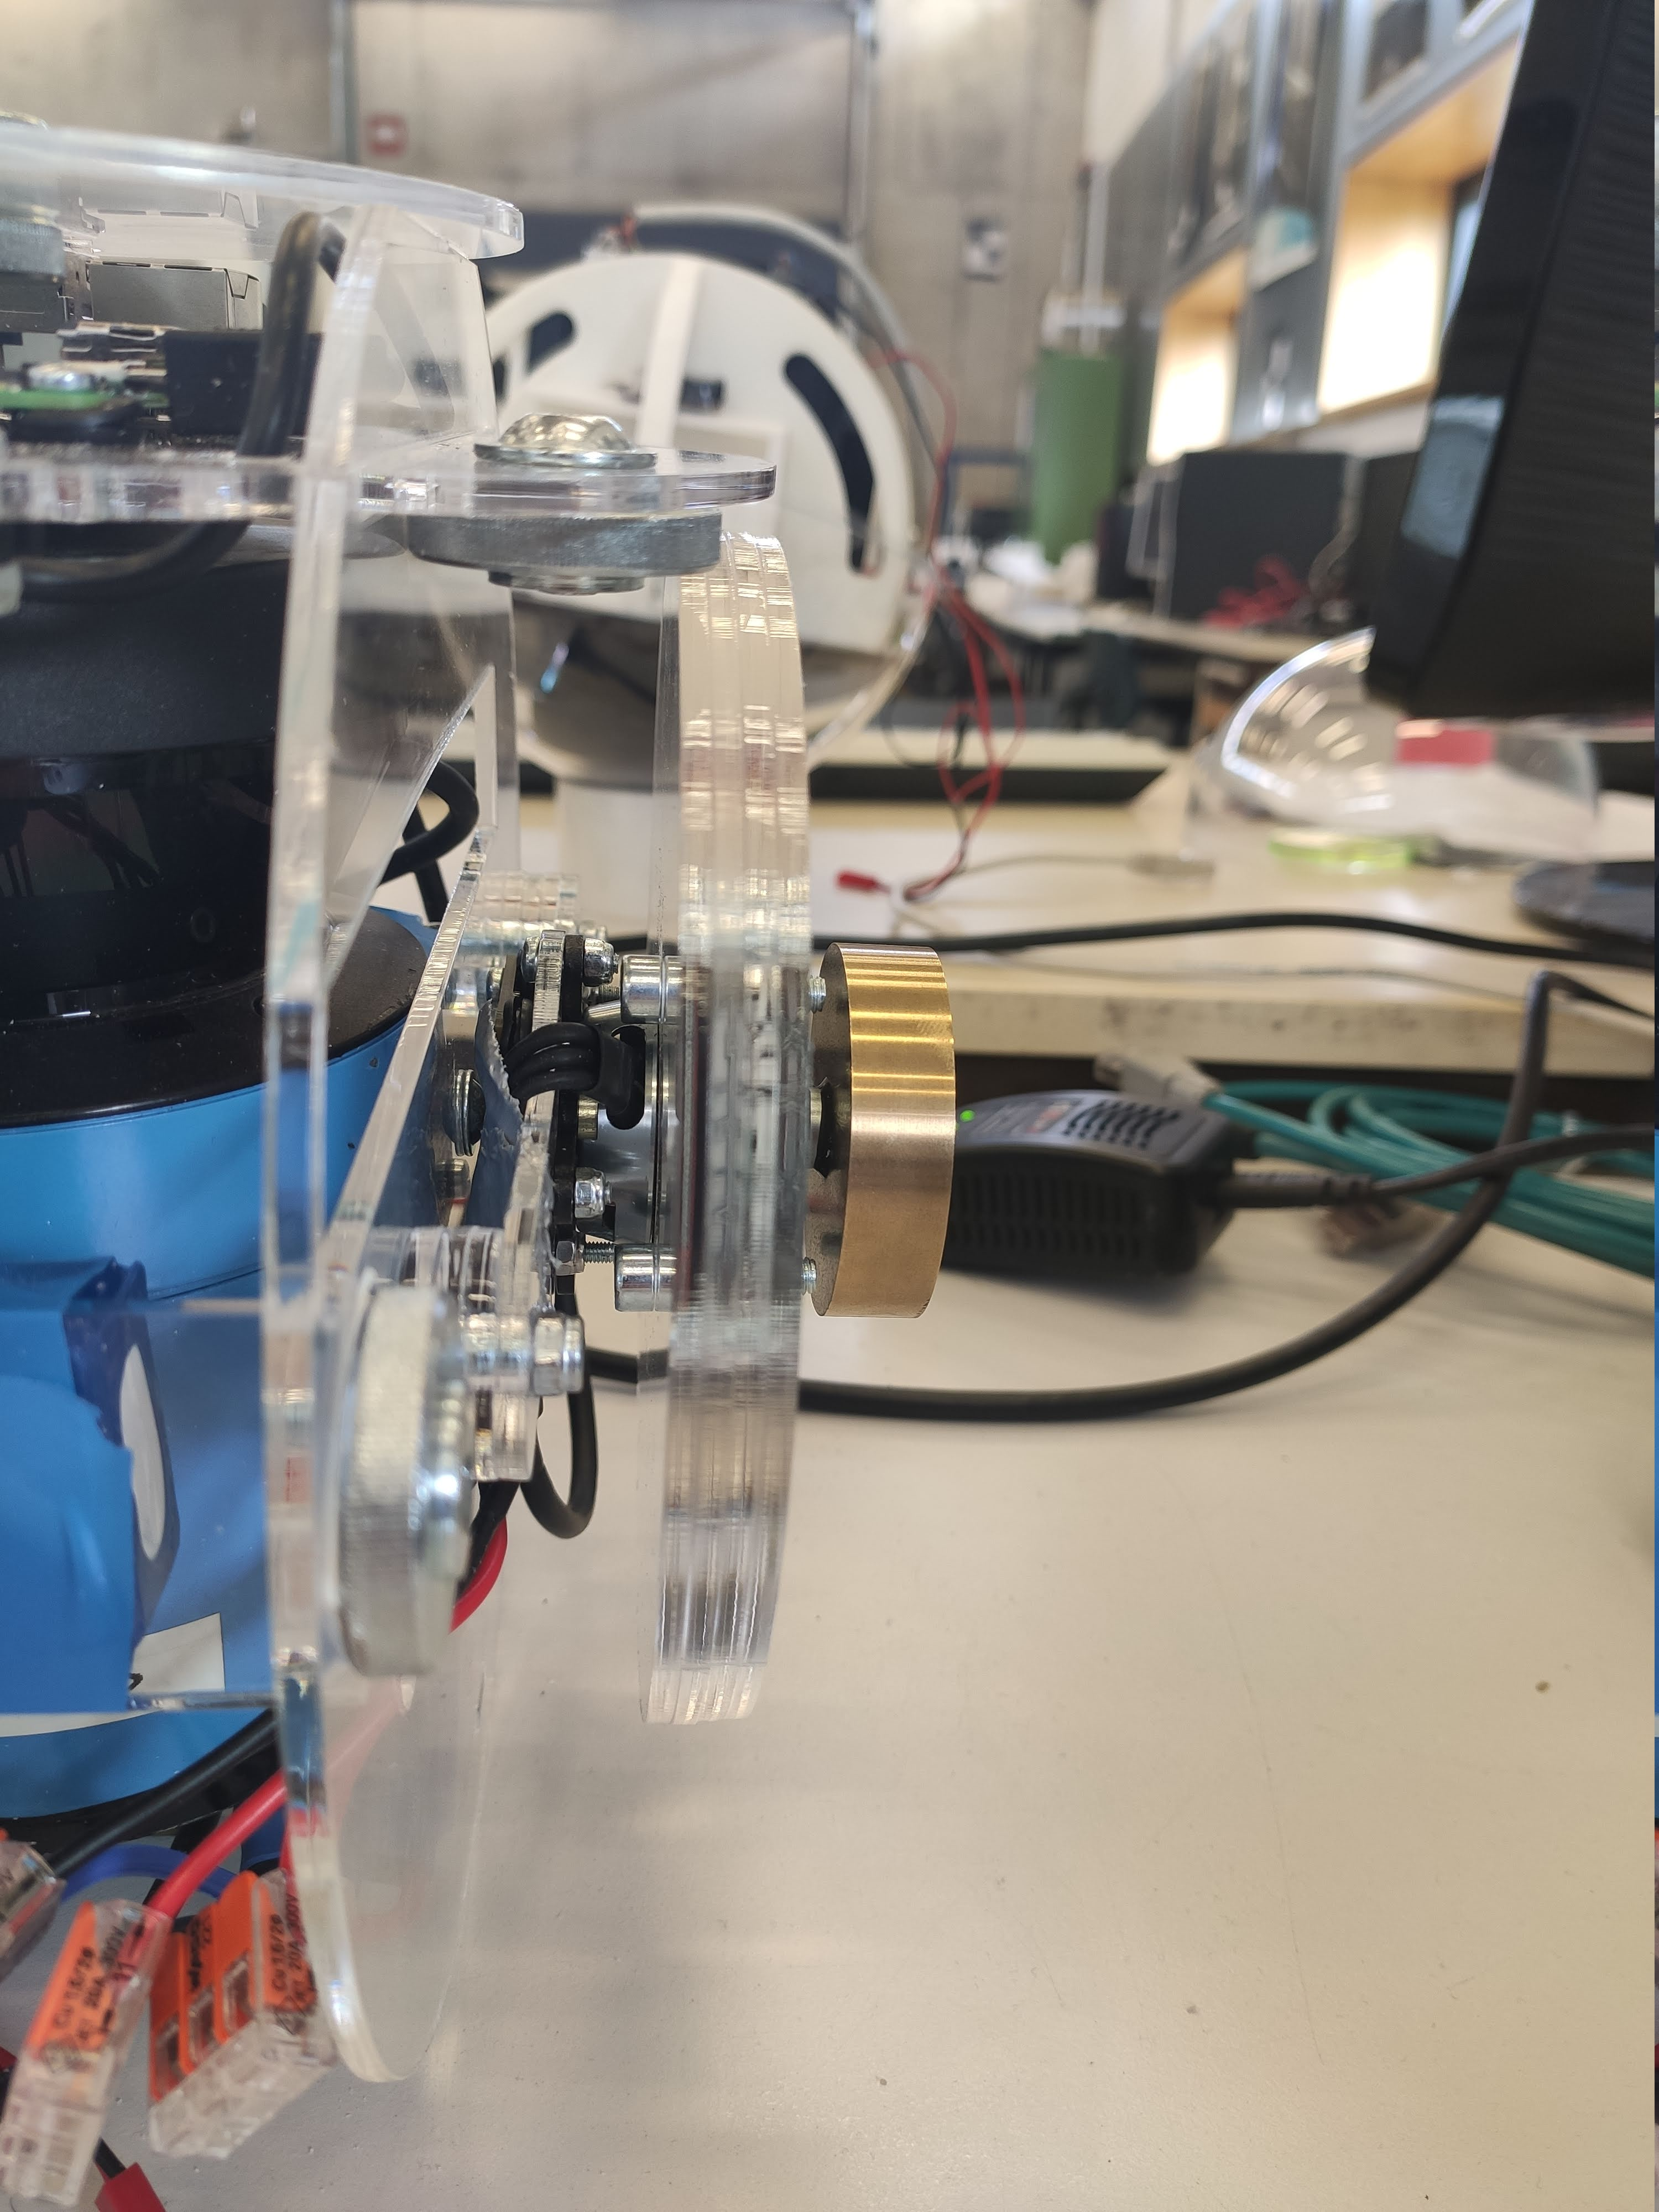
\includegraphics[width=\textwidth]{../Media/sphereRightMotor.jpg}
        \caption{IMU (beneath supporting structure) and brushless motor (above supporting structure) of the L.U.N.A sphere without shell, including flywheel mass. }
        \label{sec:TechnicalApproach:fig:motor}
\end{subfigure}
\\
\caption{Hardware setup of the L.U.N.A sphere prototype, including notches in the shell and friction granule.}
\end{figure}

Figure \ref{sec:TechnicalApproach:fig:prototype} shows the final hardware setup of the robot. In order to reduce complexity with respect to the 3D-transformation calculations, the laserscanner was placed at the center of a spherical acrylic glass shell as close as possible. This limits the laser scanners movement to rotational movement and removes translational movement completely. With this initial setup given the only room left for the acrylic glass structural components, batteries, boardcomputer, IMUs, motors, weights and wiring are the spacings between the scanner and the shell. Figure \ref{sec:TechnicalApproach:fig:motor} shows one Turnigy Park480 Brushless Outrunner motor \cite{turnigymotor} of the COAM drive with two flywheels attached. Strong epoxy glue attaches the weights to the motor shafts. As the flywheels start spinning with respect to the structural components of the sphere, the sphere itself starts spinning with respect to the ground. 

\subsection{Hardware Setup}
\label{sec:TechnicalApproach:HardwareSetup}

Figure \ref{sec:TechnicalApproach:fig:prototype} also shows that the top and the bottom of the shell are covered in salt, which made a good granule to increase friction to the ground in the early testing phase. Furthermore, there are notches in the front side of the shell to increase permeability for the laser. Unfortunately, the laser scanner measurements are still very much affected by blockades due to components of the sphere. Specifically, the outside shell is a strongly inhibiting factor as an object with the distance of the radius is measured at all times.
                                                                                                                                                                                                                  
\begin{figure}                                                                                                                                                                                                    
\centering                                                                                                                                                                                                        
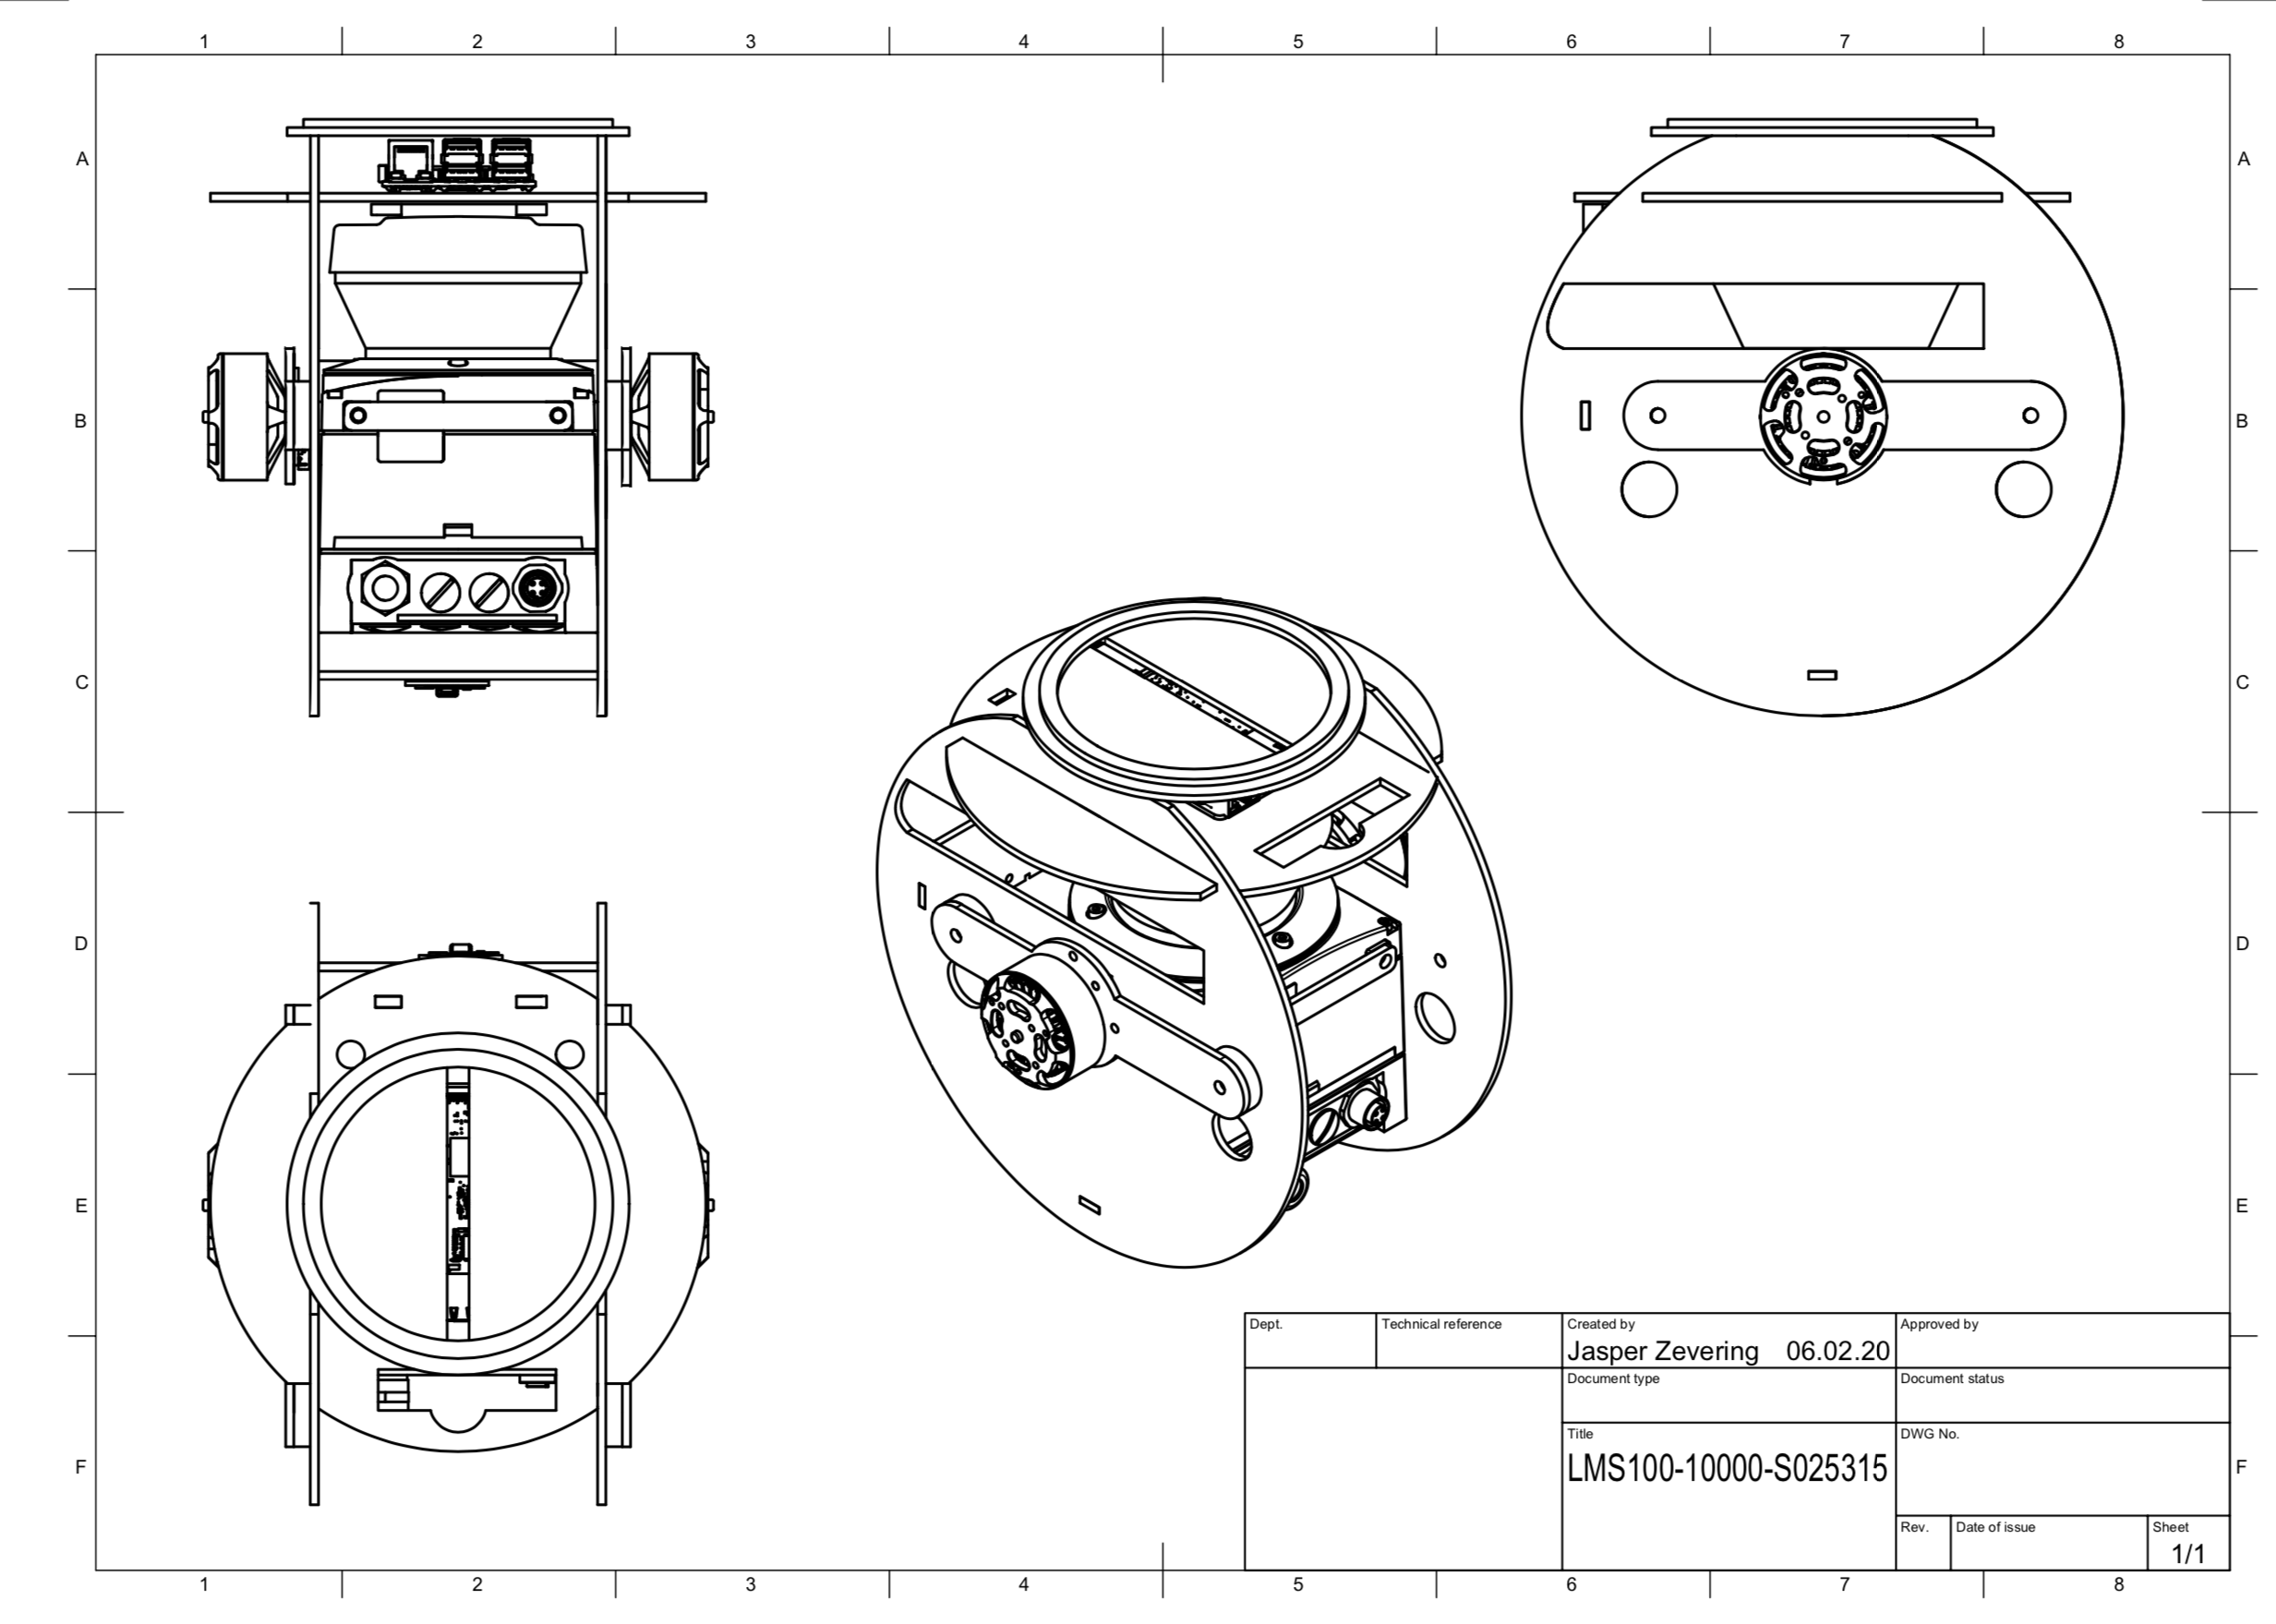
\includegraphics[width=\textwidth]{../Media/BlueprintPNG.png}                                                                                                                                                      
\caption{Blueprint that shows the mechanical structure of the spherical robot.}                                                                                                                                   
\label{sec:TechnicalApproach:fig:blueprint}                                                                                                                                                                       
\end{figure}                                                                                                                                                                                                      
                                                                                                                                                                                                                  
Figure \ref{sec:TechnicalApproach:fig:blueprint} shows a CAD blueprint about the rough interior layout of the mechanical structure of the L.U.N.A sphere, ignoring flyweights and wiring. The blueprint shows that the payload is mounted to supporting structural components which are made of acrylic glass. The raspberry pi model 3 boardcomputer is placed on top of the laser. Above that, another supporting structure can hold additional counterweights to correct for unhomogeneous weight distribution or an off place center of mass.                                                                                                     
The battery finds its place in front of the laserscanner on another supporting structure. The two brushless motors were each placed on one side of the supporting structure with spacers that leave room for the side IMU underneath one of the motors. Two other IMUs are placed in front of and beneath the laser to ensure coverage of all axes.                                                                                 
                                                                                                                                                                                                                  
\subsection{Sensor Integration}                                                                                                                                                                                   
\label{sec:TechnicalApproach:SensorIntegration}

\begin{figure}                                                                                                                                                                                                    
\centering
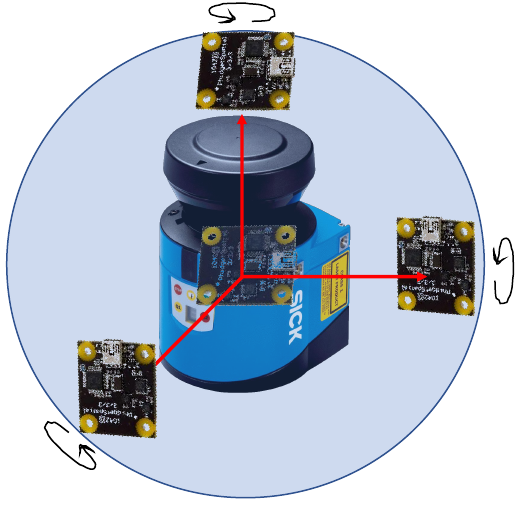
\includegraphics[width=0.5\textwidth]{../Media/virtualIMU.png}                                                                                                                                                      
\caption{Sketch that helps illustrate the combination of 3 IMUs into 1 virtual IMU that simulates being in the center of the sphere.}                                                                                                                           
\label{sec:SensorIntegration:fig:virtual}                                                                                                                                                                       
\end{figure}                                                                                                                                                                                                      

The sensor integration was fully implemented with the Robot Operating System (ROS) that has been installed on a default ubunty running on a rasperry pi 3.
Overall, three seperate PhidgetsSpacial 10441B IMUs \cite{imuphidgets} have been used to keep track of the spheres pose. Figure \ref{sec:SensorIntegration:fig:virtual} helps illustrate why three IMUs are used instead of just one. A previous study has shown that transforming the data of only one non-centered IMU leads to less quality measurements. However, combining the measurements of three IMUs, where each of which measures only the static rotation around one of their rotation axis (which also represents a rotation axis of the sphere), leads to better results. Each IMU is perpendicular to the other two, so combining the axis measurements leads to a "virtual" IMU, that simulates beeing an IMU that takes measurements from the middle of the sphere, making precise rotation speed measurements possible. 

The IMUs also ship with accelerometers that are used to determine the full pose of the sphere. Each IMU calculates their pose seperatly, using a quaternion extended kalman filter (QEKF). However, combining those poses into one did not have any positive effect, but only made the software more resource demanding and slow. Thats why only the pose of the bottom IMUs accelerometers are used to keep track of the pose.

The motors have first been accessed with the wiringPi library for raspberry pi. This library may seemed like a good prototyping library with fast results, but a switch to the more advanced piGPIO library allowed a higher throttle resolution. 

Unfortunately, the brass weights were not drilled in the very center, causing an imbalance when rotating. The resulting vibrations inhibit the movement of the sphere thus a controller was implemented that measures the extent of the vibrations using standard deviations of the IMUs axis that are not rolled over and adjusts the throttle of the motors accordingly. This was done with a simple two-point controller with hysteresis which already leads to satisfying results. The second approach of a PID controller for not letting the vibrations getting beyond the upper threshold of the hysteresis controller failed because no satisfying method of differing the normal vibrations during rolling from vibrations which leads to stopping by slipping was found. Considering the velocity of the sphere is not possible, because the speed of the sphere is calculated by the rotating speed and therefore slip of the sphere does not detect translational deceleration. 



